\documentclass[a4paper]{article}

\usepackage[UTF8]{ctex}
\usepackage[a4paper,margin=1in]{geometry}
\usepackage{graphicx}
\usepackage{float}
\usepackage{listings}
\usepackage{longtable}
\usepackage{booktabs}
\usepackage{hyperref}
\usepackage{fancyhdr}
\usepackage{lastpage}
\usepackage{color}
\usepackage{indentfirst}        % 首段缩进
\setlength{\parindent}{2em}     % 缩进2字符
\usepackage{zhnumber}           % 中文编号
\usepackage[dvipsnames]{xcolor}

%\newcommand{\college}{中山大学计算机学院}
\newcommand{\projname}{数据库系统原理实验|实验六}
\newcommand{\reporttitle}{数据库触发器实验}
\newcommand{\stuno}{23336179}
\newcommand{\authorname}{马福泉}
\newcommand{\major}{计算机科学与技术}
\newcommand{\adviser}{赖韩江}
\newcommand{\startdate}{2025年10月30日}
\newcommand{\labenddate}{2025年10月31日}
\newcommand{\labroom}{B202}

\pagestyle{fancy} % 使用 fancyhdr 风格
\fancyhf{}      % 清空默认的页眉页脚

% 设置页眉
\fancyhead[L]{\kaishu \projname}      % 左侧页眉显示项目名称
\fancyhead[C]{\kaishu \reporttitle}    % 中间页眉显示报告标题
\fancyhead[R]{\kaishu \authorname} % 右侧页眉显示作者姓名

% 设置页脚
\fancyfoot[C]{第 \thepage 页，共 \pageref{LastPage} 页} % 中间页脚显示页码

% 去除页眉页脚与正文之间的分隔线
\renewcommand{\headrulewidth}{0.4pt}
\renewcommand{\footrulewidth}{0pt}

% 设置文档背景颜色
\definecolor{mybgcolor}{RGB}{0, 0, 0} % 定义背景颜色
\definecolor{NavyBlue}{RGB}{0,0,128} % 添加颜色定义
% \pagecolor{mybgcolor} % 设置背景颜色

% listing 配置rust
% \lstdefinelanguage{Rust}{
%   keywords={fn, let, mut, struct, enum, impl, pub, use, mod, trait, where},
%   keywordstyle=\color{NavyBlue},
%   comment=[l]{//},
%   commentstyle=\color{gray},
% }
% \lstset{language=Rust}

\lstset{
  basicstyle=\ttfamily\small,
  keywordstyle=\color{NavyBlue},
  commentstyle=\color{gray},
  stringstyle=\color{red},
  showstringspaces=false,
  extendedchars=false, % 关键：不处理中文
  breaklines=true
}

\begin{document}

% 封面
\begin{titlepage}
    \centering
    
\includegraphics[width=10cm]{img/SYSULogo.png}

    \vspace{1em}
    %{\Large \college \par}
    \vspace{1em}
    {\Large \kaishu \projname \par}
    \vspace{3em}

    

    
    {\fontsize{40pt}{42pt}\kaishu \selectfont \boldmath \reporttitle\par}
    \vspace*{\fill}

    \begin{center}
    {\Large
    \makebox[5em][s]{学号}:\underline{\makebox[15em][c]{\kaishu \stuno}}\\[1em]
    \makebox[5em][s]{姓名}:\underline{\makebox[15em][c]{\kaishu \authorname}}\\[1em]
    \makebox[5em][s]{专业}:\underline{\makebox[15em][c]{\kaishu \major}}\\[1em]
    \makebox[5em][s]{课程教师}:\underline{\makebox[15em][c]{\kaishu \adviser}}\\[1em]
    \makebox[5em][s]{起始日期}:\underline{\makebox[15em][c]{\kaishu \startdate}}\\[1em]
    \makebox[5em][s]{结束日期}:\underline{\makebox[15em][c]{\kaishu \labenddate}}\\[1em]
    \makebox[5em][s]{实验地点}:\underline{\makebox[15em][c]{\kaishu \labroom}}
    }
    \end{center}

    \vspace*{\fill}
\end{titlepage}

% 目录
\tableofcontents
\newpage


\section{实验概述}

\subsection{实验目的}

通过实验加深对数据完整性的理解，学会创建和使用触发器。

\subsection{实验内容}

1. 创建一个触发器，当插入、更新或删除借阅记录表record的数据行时，能同时更新图书表book中借阅次数interview\_times
2. 创建AFTER UPDATE触发器，实现当修改读者表reader中的reader\_department数据时，打印提示（例如修改李媛媛的reader\_department为计算机系时，得到的提示是"修改数据读者名：李媛媛；修改前：经济管理系；修改后：计算机系"）
3. 创建AFTER INSERT触发器，实现禁止向图书表book插入数据的功能
4. 创建触发器，用于实现如果修改了读者表reader中的数据时，显示"已修改reader表的数据"的消息，否则返回"不存在要修改的数据或未修改数据"
5. 分别创建INSTEAD OF和AFTER 触发器，当修改图书表中book\_price的价格为原价的90\%\~{}120\%之间时，才允许修改，并显示修改后的价格变化（例如涨价了7.5\%），否则显示"价格变动太大"。 （了解两类触发器的区别）
6. 写SQL语句来验证上面1-5的触发器是否起作用。
7. 删除2，3的触发器

\section{实验报告}

\subsection{任务1：创建借阅次数更新触发器}

\subsubsection{实验步骤}

创建触发器，当对借阅记录表record进行插入、更新或删除操作时，自动更新图书表book中的借阅次数interview\_times字段。

\subsubsection{SQL代码}

\begin{lstlisting}[language=SQL]
CREATE TRIGGER tr_update_interview_times    -- 创建触发器：更新借阅次数
ON record
AFTER INSERT, UPDATE, DELETE
AS
BEGIN
    IF EXISTS(SELECT * FROM inserted)    -- 处理插入操作
    BEGIN
        UPDATE book 
        SET interviews_times = interviews_times + 1
        WHERE book_id IN (SELECT book_id FROM inserted)
    END
    
    IF EXISTS(SELECT * FROM deleted) AND NOT EXISTS(SELECT * FROM inserted)    -- 处理删除操作
    BEGIN
        UPDATE book 
        SET interviews_times = interviews_times - 1
        WHERE book_id IN (SELECT book_id FROM deleted)
    END
END
\end{lstlisting}

\subsubsection{实验结果}

\begin{lstlisting}[language=SQL]
SELECT name, type_desc, is_disabled     -- 查询触发器是否创建成功
FROM sys.triggers 
WHERE name = 'tr_update_interview_times';

SELECT book_id, book_name, interviews_times     -- 查看触发器执行前的借阅次数
FROM book 
WHERE book_id = 'b0001';

INSERT INTO record (reader_id, book_id, borrow_date, return_date, notes)    -- 插入借阅记录触发器
VALUES ('r0001', 'b0001', '2024-01-01', '2024-01-15', NULL);

SELECT book_id, book_name, interviews_times     -- 查看触发器执行后的借阅次数
FROM book 
WHERE book_id = 'b0001';
\end{lstlisting}

% 截图预留空间
\begin{figure}[H]
    \centering
    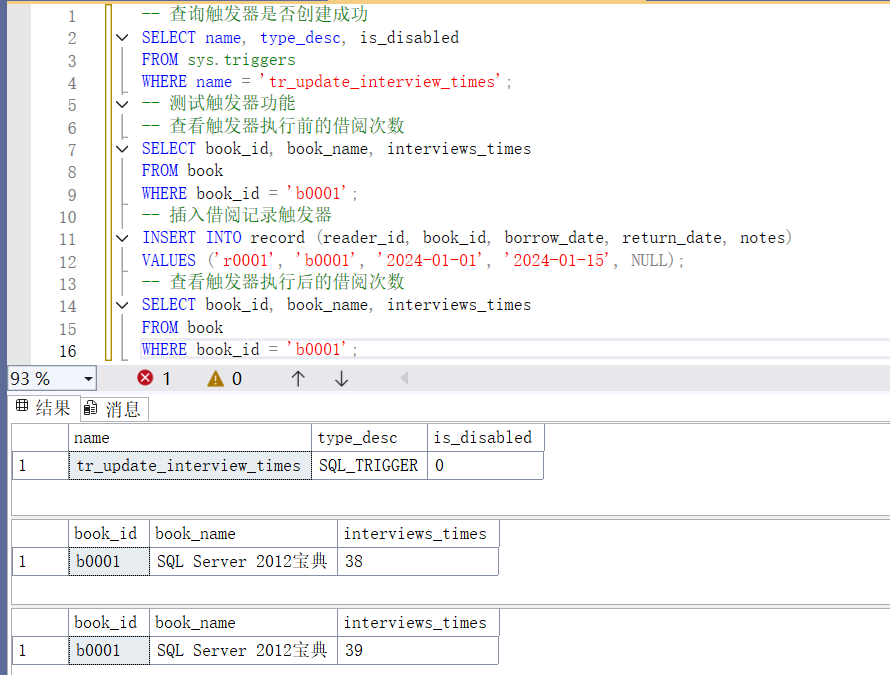
\includegraphics[width=0.8\textwidth]{img/task1.png}
    \caption{触发器创建结果截图}
\end{figure}

\subsection{任务2：创建读者部门修改提示触发器}

\subsubsection{实验步骤}

创建AFTER UPDATE触发器，当修改读者表reader中的reader\_department数据时，打印相应的提示信息。

\subsubsection{SQL代码}

\begin{lstlisting}[language=SQL]
CREATE TRIGGER tr_reader_department_update    -- 创建触发器：读者部门修改提示
ON reader
AFTER UPDATE
AS
BEGIN
    IF UPDATE(reader_department)
    BEGIN
        DECLARE @reader_name NVARCHAR(50)
        DECLARE @old_dept NVARCHAR(50)
        DECLARE @new_dept NVARCHAR(50)
        
        SELECT @reader_name = i.reader_name,
               @old_dept = d.reader_department,
               @new_dept = i.reader_department
        FROM inserted i
        INNER JOIN deleted d ON i.reader_id = d.reader_id
        
        PRINT '修改数据读者名：' + @reader_name + '；修改前：' + @old_dept + '；修改后：' + @new_dept
    END
END
\end{lstlisting}

\subsubsection{实验结果}

\begin{lstlisting}[language=SQL]
SELECT name, type_desc, is_disabled     -- 查询触发器是否创建成功
FROM sys.triggers 
WHERE name = 'tr_reader_department_update';

SELECT reader_id, reader_name, reader_department     -- 查看修改前的读者信息
FROM reader 
WHERE reader_name = '李媛媛';

UPDATE reader     -- 执行修改操作，触发器会输出提示信息
SET reader_department = '计算机系' 
WHERE reader_name = '李媛媛';

SELECT reader_id, reader_name, reader_department     -- 查看修改后的读者信息
FROM reader 
WHERE reader_name = '李媛媛';
\end{lstlisting}

% 截图预留空间
\begin{figure}[H]
    \centering
    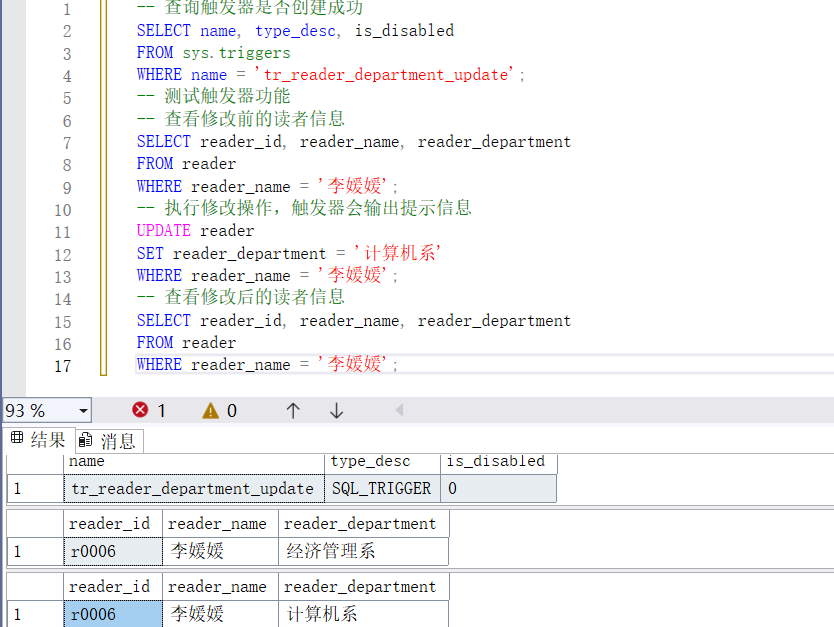
\includegraphics[width=0.8\textwidth]{img/task2.png}
    \caption{读者部门修改触发器结果截图}
\end{figure}

\subsection{任务3：创建禁止插入图书数据触发器}

\subsubsection{实验步骤}

创建AFTER INSERT触发器，实现禁止向图书表book插入数据的功能。

\subsubsection{SQL代码}

\begin{lstlisting}[language=SQL]
CREATE TRIGGER tr_prevent_book_insert    -- 创建触发器：禁止插入图书数据
ON book
AFTER INSERT
AS
BEGIN
    ROLLBACK TRANSACTION
    PRINT '禁止向图书表插入数据!'
END
\end{lstlisting}

\subsubsection{实验结果}

\begin{lstlisting}[language=SQL]
SELECT name, type_desc, is_disabled     -- 查询触发器是否创建成功
FROM sys.triggers 
WHERE name = 'tr_prevent_book_insert';

SELECT COUNT(*) AS book_count FROM book;    -- 查看插入前的图书数量

INSERT INTO book (book_id, book_name, book_isbn, book_author, book_publisher, book_price, interviews_times)
VALUES ('b1000', '测试图书', '978-3-16-148410-0', '测试作者', '测试出版社', 50.00, 0);  -- 尝试插入数据

SELECT COUNT(*) AS book_count FROM book;    -- 查看插入后的图书数量（应该没有变化）
\end{lstlisting}

% 截图预留空间
\begin{figure}[H]
    \centering
    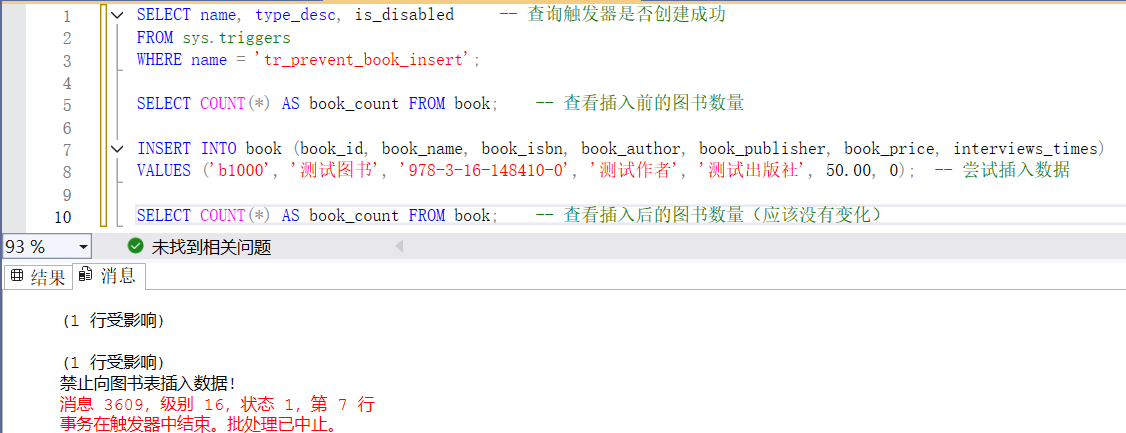
\includegraphics[width=0.8\textwidth]{img/task3.png}
    \caption{禁止插入触发器结果截图}
\end{figure}

\subsection{任务4：创建读者表修改状态提示触发器}

\subsubsection{实验步骤}

创建触发器，用于实现如果修改了读者表reader中的数据时，显示相应的消息提示。

\subsubsection{SQL代码}

\begin{lstlisting}[language=SQL]
CREATE TRIGGER tr_reader_update_status    -- 创建触发器：读者表修改状态提示
ON reader
AFTER UPDATE
AS
BEGIN
    IF @@ROWCOUNT > 0
    BEGIN
        PRINT '已修改reader表的数据'
    END
    ELSE
    BEGIN
        PRINT '不存在要修改的数据或未修改数据'
    END
END
\end{lstlisting}

\subsubsection{实验结果}

\begin{lstlisting}[language=SQL]
SELECT name, type_desc, is_disabled     -- 查询触发器是否创建成功
FROM sys.triggers 
WHERE name = 'tr_reader_update_status';

SELECT reader_id, reader_name, reader_sex     -- 查看修改前的读者信息
FROM reader 
WHERE reader_id = 'r0001';

UPDATE reader     -- 执行修改操作，触发器会输出状态信息
SET reader_sex = '女' 
WHERE reader_id = 'r0001';

SELECT reader_id, reader_name, reader_sex     -- 查看修改后的读者信息
FROM reader 
WHERE reader_id = 'r0001';

UPDATE reader     -- 测试修改不存在的数据
SET reader_sex = '男' 
WHERE reader_id = 'r9999';
\end{lstlisting}

% 截图预留空间
\begin{figure}[H]
    \centering
    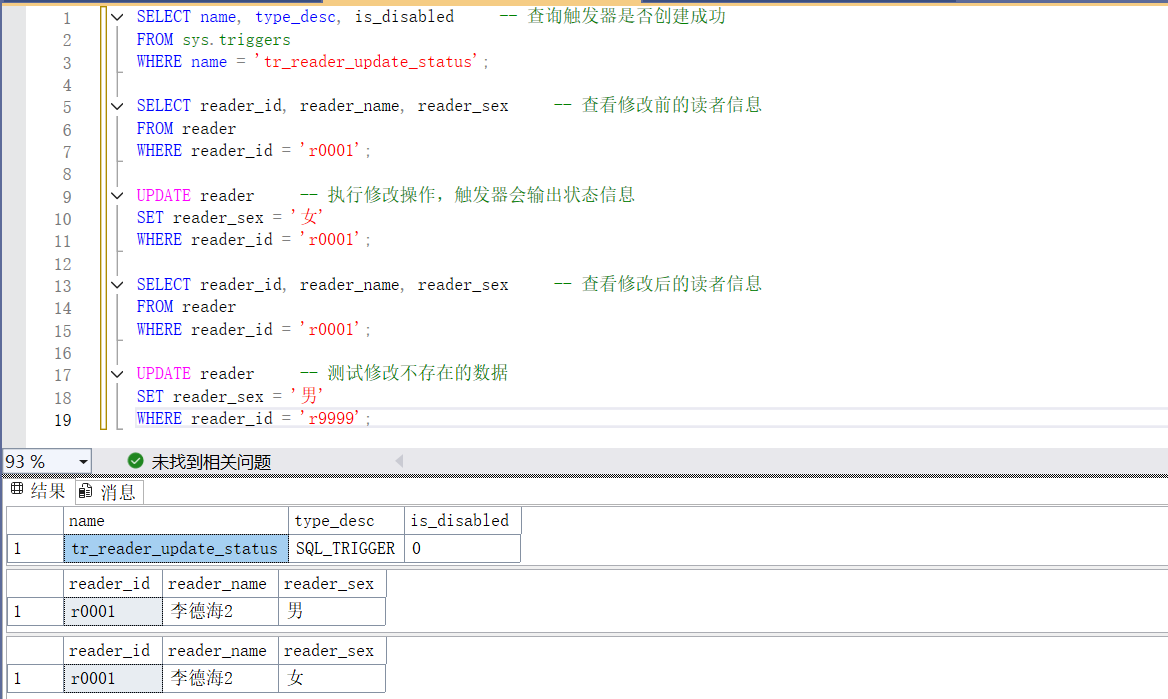
\includegraphics[width=0.8\textwidth]{img/task4_1.png}
    \caption{读者表修改状态触发器结果截图一}
\end{figure}
\begin{figure}[H]
    \centering
    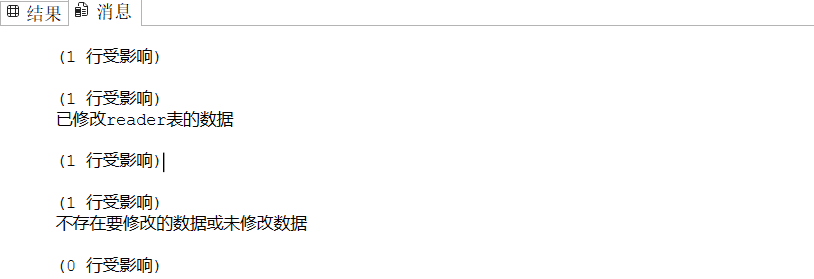
\includegraphics[width=0.8\textwidth]{img/task4_2.png}
    \caption{读者表修改状态触发器结果截图二}
\end{figure}
\subsection{任务5：创建图书价格修改控制触发器}

\subsubsection{实验步骤}

分别创建INSTEAD OF和AFTER触发器，控制图书价格的修改范围在原价的90\%\~{}120\%之间。

\subsubsection{SQL代码}

\begin{lstlisting}[language=SQL]
IF OBJECT_ID('v_book_price', 'V') IS NOT NULL
    DROP VIEW v_book_price;
GO

-- 创建视图
CREATE VIEW v_book_price AS
SELECT book_id, book_name, book_price, book_author, book_publisher
FROM book;
GO

-- 创建INSTEAD OF触发器
CREATE TRIGGER tr_book_price_instead_of
ON v_book_price
INSTEAD OF UPDATE
AS
BEGIN
    DECLARE @book_id NVARCHAR(10);
    DECLARE @old_price DECIMAL(10,2);
    DECLARE @new_price DECIMAL(10,2);
    DECLARE @price_change_rate DECIMAL(5,2);
    
    SELECT @book_id = i.book_id,
           @old_price = d.book_price,
           @new_price = i.book_price
    FROM inserted i
    INNER JOIN deleted d ON i.book_id = d.book_id;
    
    SET @price_change_rate = (@new_price - @old_price) / @old_price * 100;
    
    IF @new_price BETWEEN @old_price * 0.9 AND @old_price * 1.2
    BEGIN
        UPDATE book 
        SET book_price = @new_price
        WHERE book_id = @book_id;
        
        IF @price_change_rate > 0
            PRINT '涨价了' + CAST(ABS(@price_change_rate) AS NVARCHAR(10)) + '%';
        ELSE
            PRINT '降价了' + CAST(ABS(@price_change_rate) AS NVARCHAR(10)) + '%';
    END
    ELSE
    BEGIN
        PRINT '价格变动太大';
    END
END;
GO

-- 创建AFTER触发器
CREATE TRIGGER tr_book_price_after
ON book
AFTER UPDATE
AS
BEGIN
    IF UPDATE(book_price)
    BEGIN
        DECLARE @book_id NVARCHAR(10);
        DECLARE @old_price DECIMAL(10,2);
        DECLARE @new_price DECIMAL(10,2);
        DECLARE @price_change_rate DECIMAL(5,2);
        
        SELECT @book_id = i.book_id,
               @old_price = d.book_price,
               @new_price = i.book_price
        FROM inserted i
        INNER JOIN deleted d ON i.book_id = d.book_id;
        
        SET @price_change_rate = (@new_price - @old_price) / @old_price * 100;
        
        IF NOT (@new_price BETWEEN @old_price * 0.9 AND @old_price * 1.2)
        BEGIN
            ROLLBACK TRANSACTION;
            PRINT '价格变动太大';
        END
        ELSE
        BEGIN
            IF @price_change_rate > 0
                PRINT '涨价了' + CAST(ABS(@price_change_rate) AS NVARCHAR(10)) + '%';
            ELSE
                PRINT '降价了' + CAST(ABS(@price_change_rate) AS NVARCHAR(10)) + '%';
        END
    END
END;
GO
\end{lstlisting}

\subsubsection{实验结果}

\begin{lstlisting}[language=SQL]
SELECT name, type_desc, is_disabled     -- 查询触发器是否创建成功
FROM sys.triggers 
WHERE name IN ('tr_book_price_instead_of', 'tr_book_price_after');

SELECT * FROM INFORMATION_SCHEMA.VIEWS WHERE TABLE_NAME = 'v_book_price';    -- 查询视图是否创建成功

SELECT book_id, book_name, book_price     -- 查看修改前的图书价格
FROM book 
WHERE book_id = 'b0001';

UPDATE book     -- 测试合理的价格变动（5%涨价）
SET book_price = 94.50 
WHERE book_id = 'b0001';

SELECT book_id, book_name, book_price     -- 查看修改后的价格
FROM book 
WHERE book_id = 'b0001';

UPDATE book     -- 测试过大的价格变动（50%涨价，应该被阻止）
SET book_price = 135.00 
WHERE book_id = 'b0001';

UPDATE v_book_price     -- 通过视图修改价格（10%涨价）
SET book_price = 99.00 
WHERE book_id = 'b0001';

SELECT book_id, book_name, book_price     -- 查看最终价格
FROM book 
WHERE book_id = 'b0001';
\end{lstlisting}

% 截图预留空间
\begin{figure}[H]
    \centering
    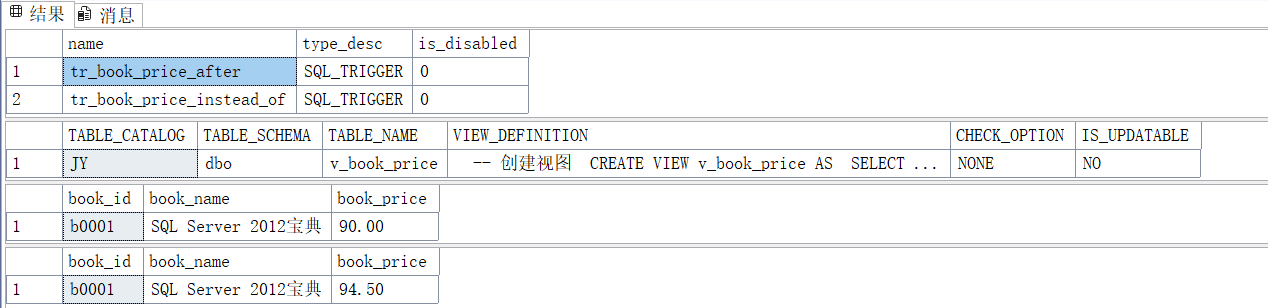
\includegraphics[width=0.8\textwidth]{img/task5_1.png}
    \caption{图书价格修改控制触发器结果截图一}
\end{figure}
\begin{figure}[H]
    \centering
    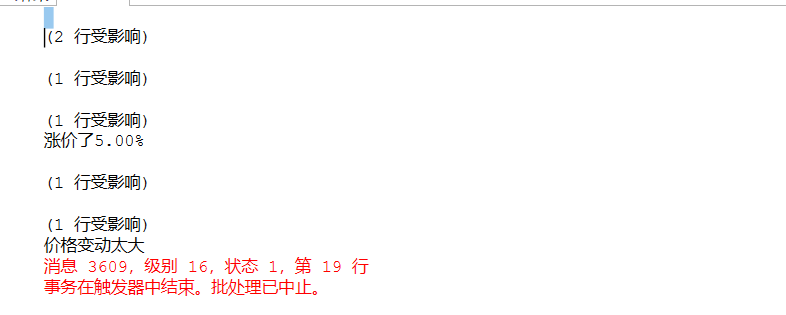
\includegraphics[width=0.8\textwidth]{img/task5_2.png}
    \caption{图书价格修改控制触发器结果截图二}
\end{figure}

\subsection{任务6：触发器功能验证}

编写SQL语句验证上述1-5个触发器的功能是否正常工作。
已经在上述实验步骤对应任务中进行了验证。


\subsection{任务7：删除指定触发器}

\subsubsection{实验步骤}

删除任务2和任务3创建的触发器。

\subsubsection{SQL代码}

\begin{lstlisting}[language=SQL]
DROP TRIGGER tr_reader_department_update;    -- 删除任务2的触发器
DROP TRIGGER tr_prevent_book_insert;    -- 删除任务3的触发器

SELECT name, type_desc, is_disabled     -- 验证触发器是否删除成功
FROM sys.triggers 
WHERE name IN ('tr_reader_department_update', 'tr_prevent_book_insert');
\end{lstlisting}

\subsubsection{实验结果}

% 截图预留空间
\begin{figure}[H]
    \centering
    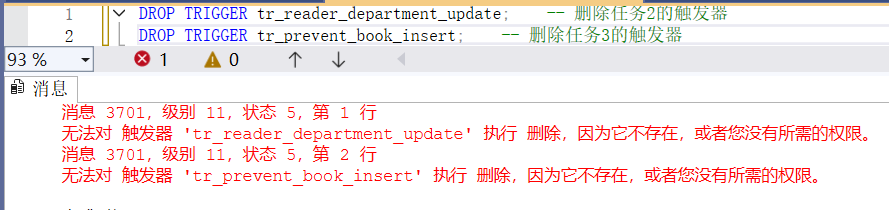
\includegraphics[width=0.8\textwidth]{img/task7.png}
    \caption{触发器删除结果截图}
\end{figure}

\section{实验总结}

通过本次实验，我深入学习了数据库触发器的创建和使用方法。主要收获包括：

1. 掌握了AFTER、INSTEAD OF等不同类型触发器的区别和应用场景

2. 学会了在触发器中使用inserted和deleted表来获取操作前后的数据

3. 理解了触发器在维护数据完整性和实现业务逻辑方面的重要作用

4. 熟悉了触发器的调试和验证方法

触发器作为数据库的重要特性，能够在数据发生变化时自动执行相应的操作，为数据库应用系统提供了强大的数据管理能力。

\end{document}